
\section[Lexical Semantics]{Computational Lexical Semanitcs}
\subsection{ }



\begin{frame}
\frametitle{Motivation}


\begin{figure}
\centering
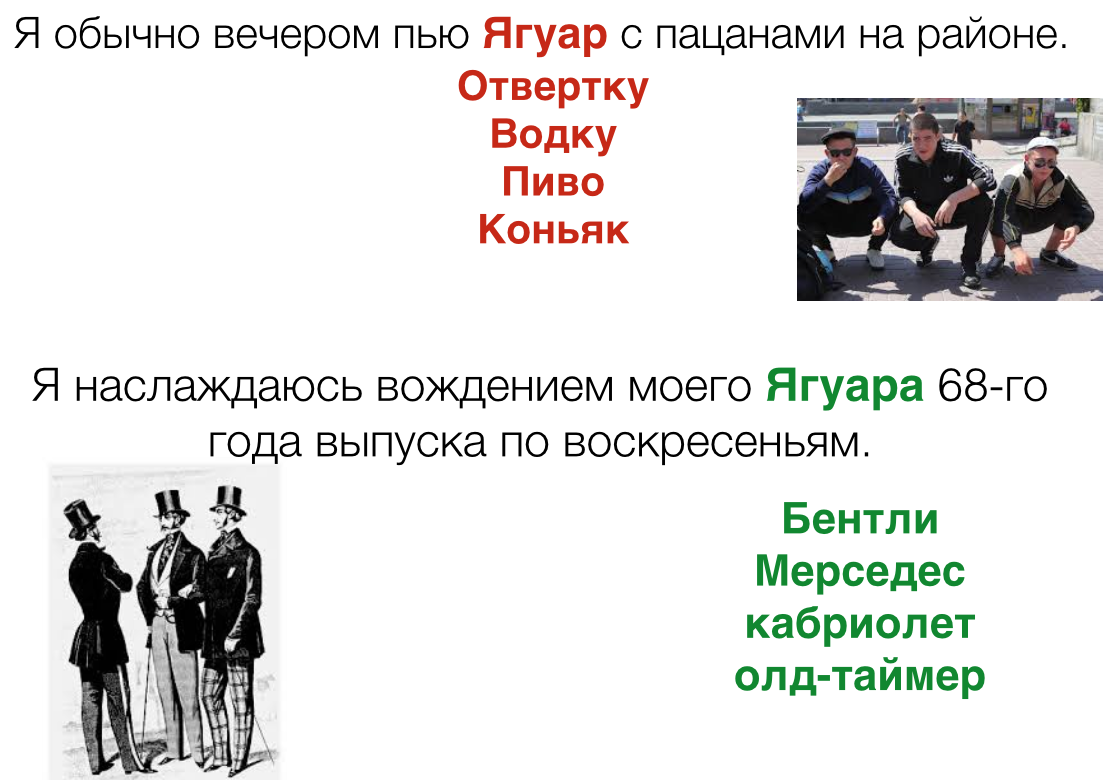
\includegraphics[width=0.95\textwidth]{./figures/jaguar}
\end{figure} 
\end{frame}


\begin{frame}
\frametitle{Two Worlds of Computational Lexical Semantics}


\begin{figure}
\centering
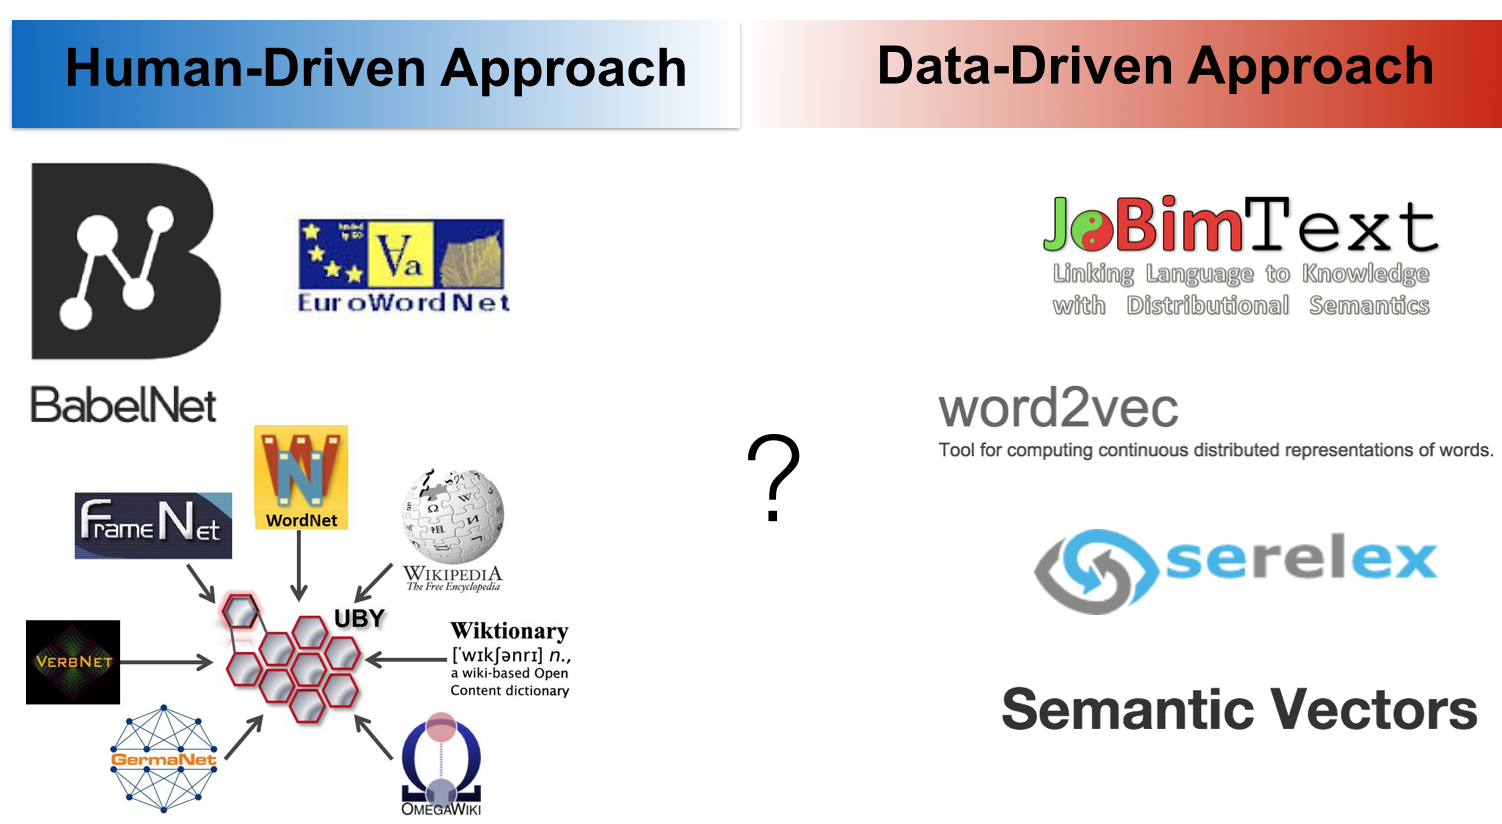
\includegraphics[width=1.0\textwidth]{./figures/two-worlds}
\end{figure} 
\end{frame}





\begin{frame}
\frametitle{Computational Lexical Semantics: Levels of Analysis}

\begin{figure}
\centering
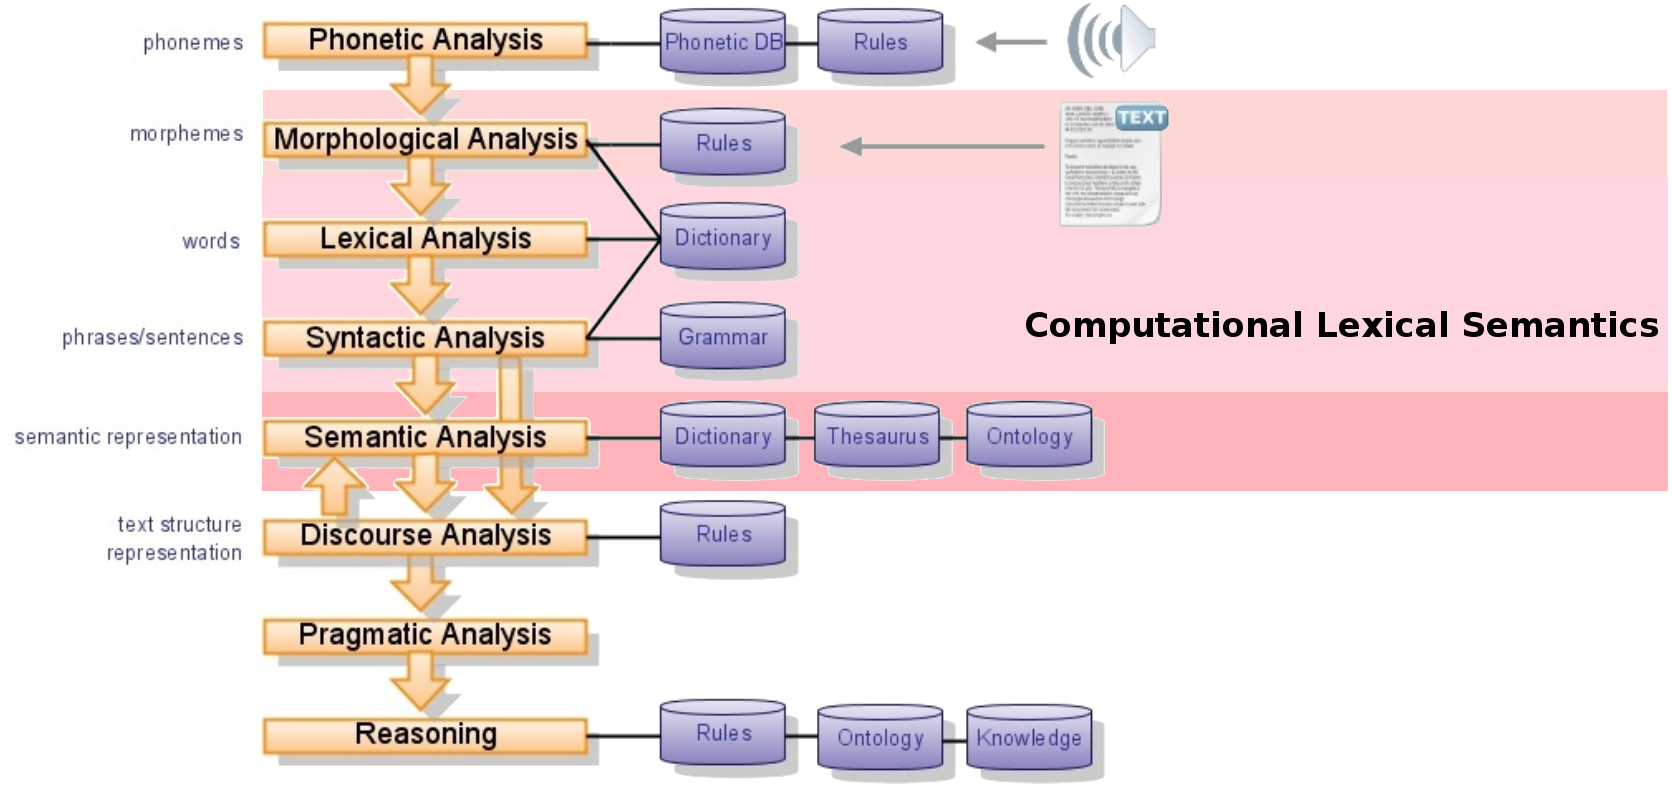
\includegraphics[width=1.05\textwidth]{figures/levels}
\end{figure}

 \tiny{* source of the image \url{http://www.uclouvain.be/en-cours-2013-LINGI2263.html}}

\end{frame}





\begin{frame}
\frametitle{Tasks}

\textbf{Computational models} of semantics of words and multiword expressions are used to solve following tasks:
 
\begin{itemize}
  \item Word sense disambiguation (WSD) and named entity disambiguation;
  \item Semantic relation extraction;
  \item Semantic similarity and semantic relatedness;
  \item Word sense induction (WSI) and discrimination;
  \item Generation of features for other NLP tasks.
\end{itemize}

\end{frame}




\begin{frame}
\frametitle{Introduction into the field}

\begin{itemize}
  \item Jurafsky D. and Martin J.H. An \textbf{Introduction to Natural Language Processing, Computational Linguistics, and Speech Recognition} (2009), chapters 19,20, 22.

\item Cruys T. \textbf{Mining for meaning: the extraction of lexico-semantic knowledge from text} (2010). PhD thesis. \url{http://dissertations.ub.rug.nl/faculties/arts/2010/t.van.de.cruys/} 

\item Panchenko A. \textbf{Similarity Measures for Semantic Relation Extraction} (2013) \url{http://cental.fltr.ucl.ac.be/team/~panchenko/thesis.pdf} 


\end{itemize}


\end{frame}



\begin{frame}
\frametitle{Key concepts}

\begin{itemize}
 \item \textbf{Lexical unit}: word, multiword expression (MWE), noun phrase (NP).
 \item \textbf{Vocabulary}: a set of words. 
 \item \textbf{Semantic relation}: defines a connection between lexical units. Relation can have a numerical weight and/or a type, such as synonymy, hypernymy, co-hyponymy or association. 
 \item \textbf{Semantic resource}: Vocabulary + a set of semantic relations. 
 \item \textbf{Distributional thesaurus}: a semantic resource without types. 
 \item \textbf{Semantic relatedness/similarity}: a numerical measure of word similarity.
 \item \textbf{Synset}: a group of mutual synonyms. 
 \item \textbf{Sense}: sense of a lexical item. 
 \item \textbf{Sense inventory:} a set of senses of a given vocabulary. 
\end{itemize}


\end{frame}



\begin{frame}
\frametitle{Semantic Resources}

\begin{block}{}

A \textbf{semantic resource} is an graph $(C, R)$:
\begin{itemize}
\item nodes $C$ represent \textbf{terms};
\item edges $R$ represent untyped \textbf{semantic relations}.
\end{itemize}

\end{block}

\begin{figure}
\centering
\includegraphics[height=0.400\textwidth]{./../figures/sr-29-example-crop2}
\end{figure}

\end{frame}




\begin{frame}
\frametitle{Semantic Relations}
\begin{figure}
\centering
\includegraphics[width=0.65\textwidth]{./../figures/sr-29-example}
\caption{A semantic resource composed of 29 relations.}
\end{figure}

\end{frame}





\begin{frame}
\frametitle{Types of semantic relaitons}

\begin{figure}
\centering
\includegraphics[height=0.49\textwidth]{./../figures/sr-example-2}
\includegraphics[height=0.35\textwidth]{./../figures/sr-example-spacer}
\includegraphics[height=0.43\textwidth]{./../figures/sr-example-untyped-2}
\caption{A semantic resource with (a) typed (b) untyped relations. }
\end{figure}

\end{frame}



\begin{frame}
\frametitle{Types of semantic relations}

\begin{figure}
\centering
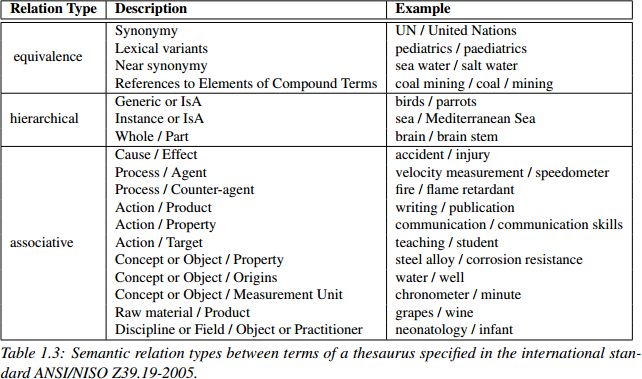
\includegraphics[height=0.49\textwidth]{./figures/sem-types}
\end{figure}

\end{frame}





\begin{frame}
\frametitle{Types of semantic relations}
\begin{figure}
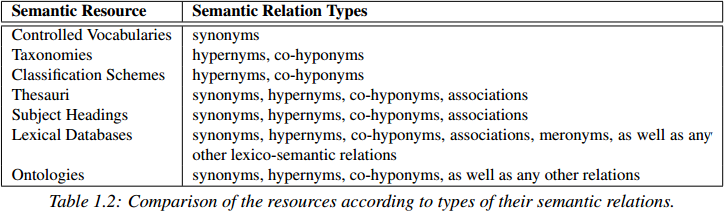
\includegraphics[width=1.0\textwidth]{figures/sem-res-table}
\end{figure}
\end{frame}







\frame{
\frametitle{Synsets}

\begin{figure}
\centering
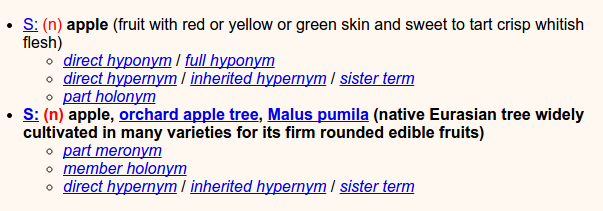
\includegraphics[width=0.9\textwidth]{figures/synset}
\caption{ WordNet synsets: \url{http://wordnetweb.princeton.edu/perl/webwn}. }
\end{figure}

}

\frame{
\frametitle{Synsets}

\begin{figure}
\centering
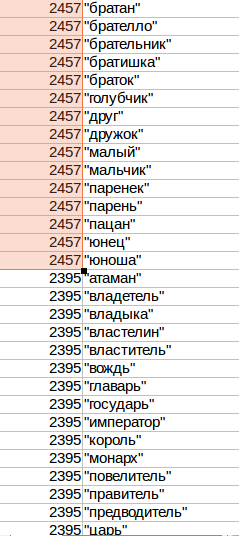
\includegraphics[width=0.26\textwidth]{figures/yarn}
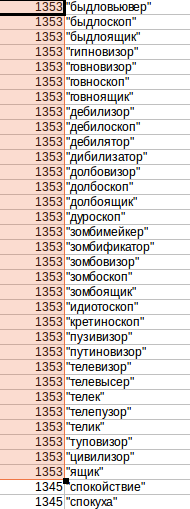
\includegraphics[width=0.22\textwidth]{figures/yarn2}
\caption{ YARN synsets: \url{http://russianword.net}. }
\end{figure}

}

\frame{
\frametitle{Synsets}

\begin{figure}
\centering
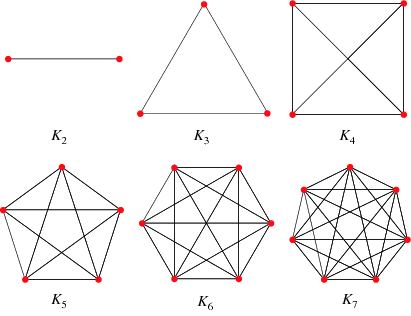
\includegraphics[width=0.7\textwidth]{figures/complete}
\caption{ Synset is a complete graph of synonyms. Source: \url{http://mathworld.wolfram.com/CompleteGraph.html}. }
\end{figure}

}

\begin{frame}
\frametitle{Semantic resources: expressiveness}

\begin{figure}
\centering
\includegraphics[width=0.9\textwidth]{../figures/expressivness}
\caption{ Expressiveness of different semantic resources. }
\label{fig:expressiveness}
\end{figure}

\end{frame}





\begin{frame}
\frametitle{Semantic resources: taxonomy }

\begin{figure}
\centering
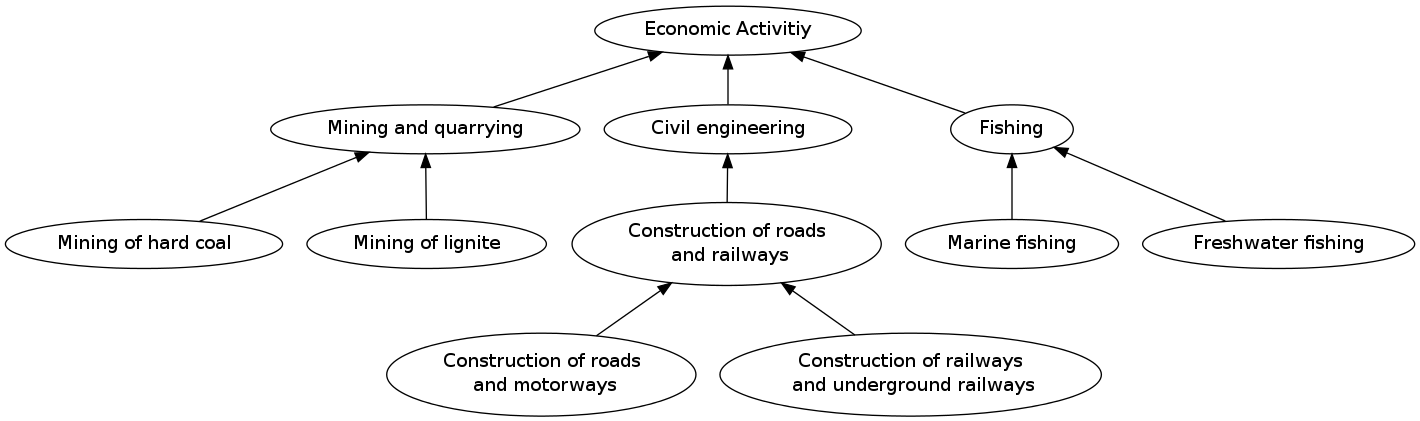
\includegraphics[width=1.0\textwidth]{figures/taxonomy-new}
\caption{ A part of the taxonomy of economical activities NACE.}
\label{fig:taxonomy}
\end{figure}

\end{frame}





\begin{frame}
\frametitle{Semantic resources: thesaurus }

\begin{figure}
\centering
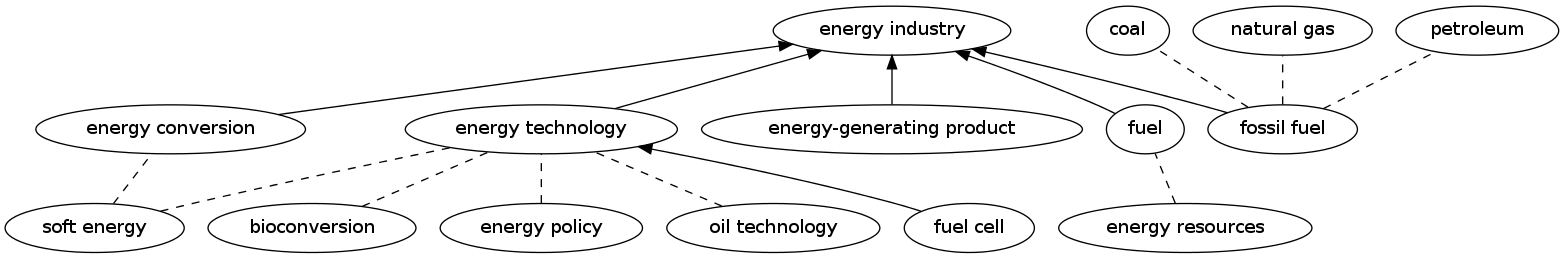
\includegraphics[width=1.0\textwidth]{figures/thesaurus-new}
\caption{ The Eurovoc thesaurus: the term ``energy industry'' and its semantic relations. Here, hypernyms are denoted with arrows and associations are denoted with dashed lines.}
\label{fig:thesaurus}
\end{figure}
\end{frame}




\begin{frame}
\frametitle{Semantic resources: lexical database }

\begin{figure}
\centering
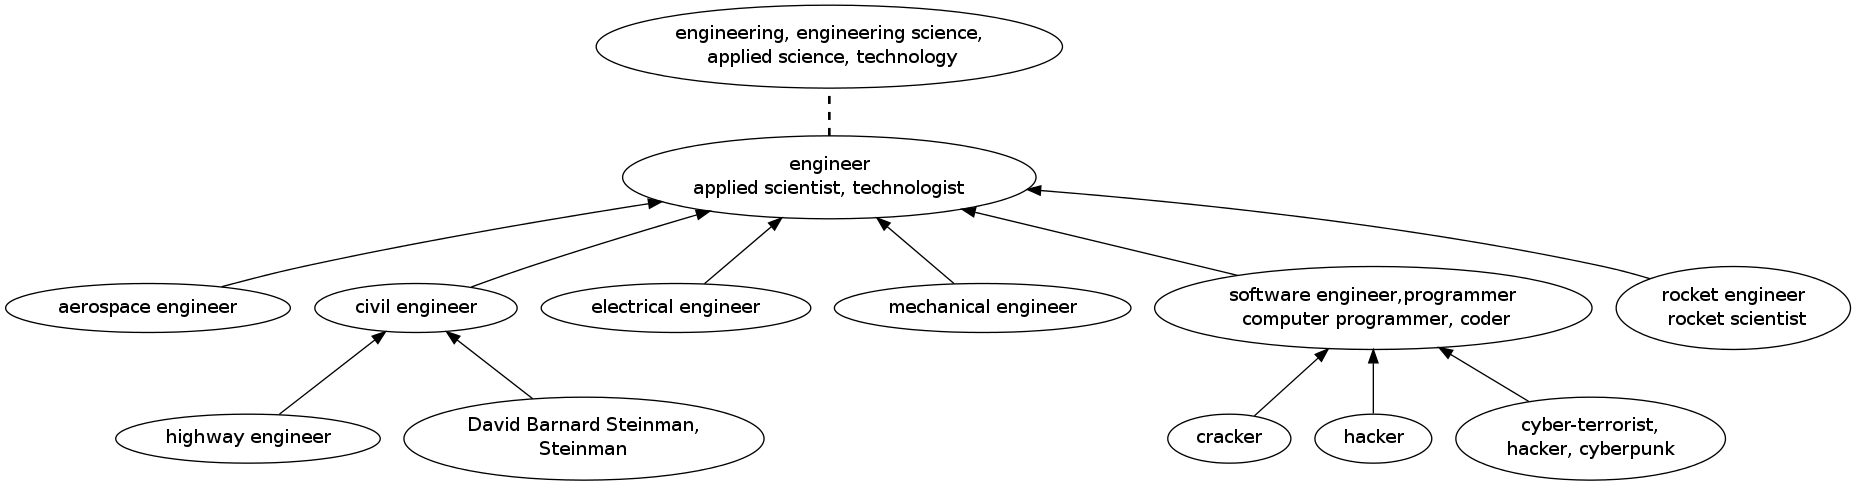
\includegraphics[width=1.0\textwidth]{figures/wordnet-new}
\caption{ Lexical database WordNet: synset \textit{engineer} and its semantic relations. }
\label{fig:wordnet}
\end{figure}
\end{frame}


\begin{frame}
\frametitle{Semantic resources: lexical database}

\begin{figure}
\centering
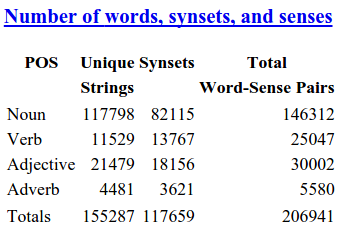
\includegraphics[width=.7\textwidth]{figures/wnstat}
\caption{ WordNet statistics. Source: \url{https://wordnet.princeton.edu/wordnet/man/wnstats.7WN.html} }
\label{fig:wordnet}
\end{figure}
\end{frame}



\begin{frame}
\frametitle{Semantic Resources: WordNet}

\begin{figure}
\centering
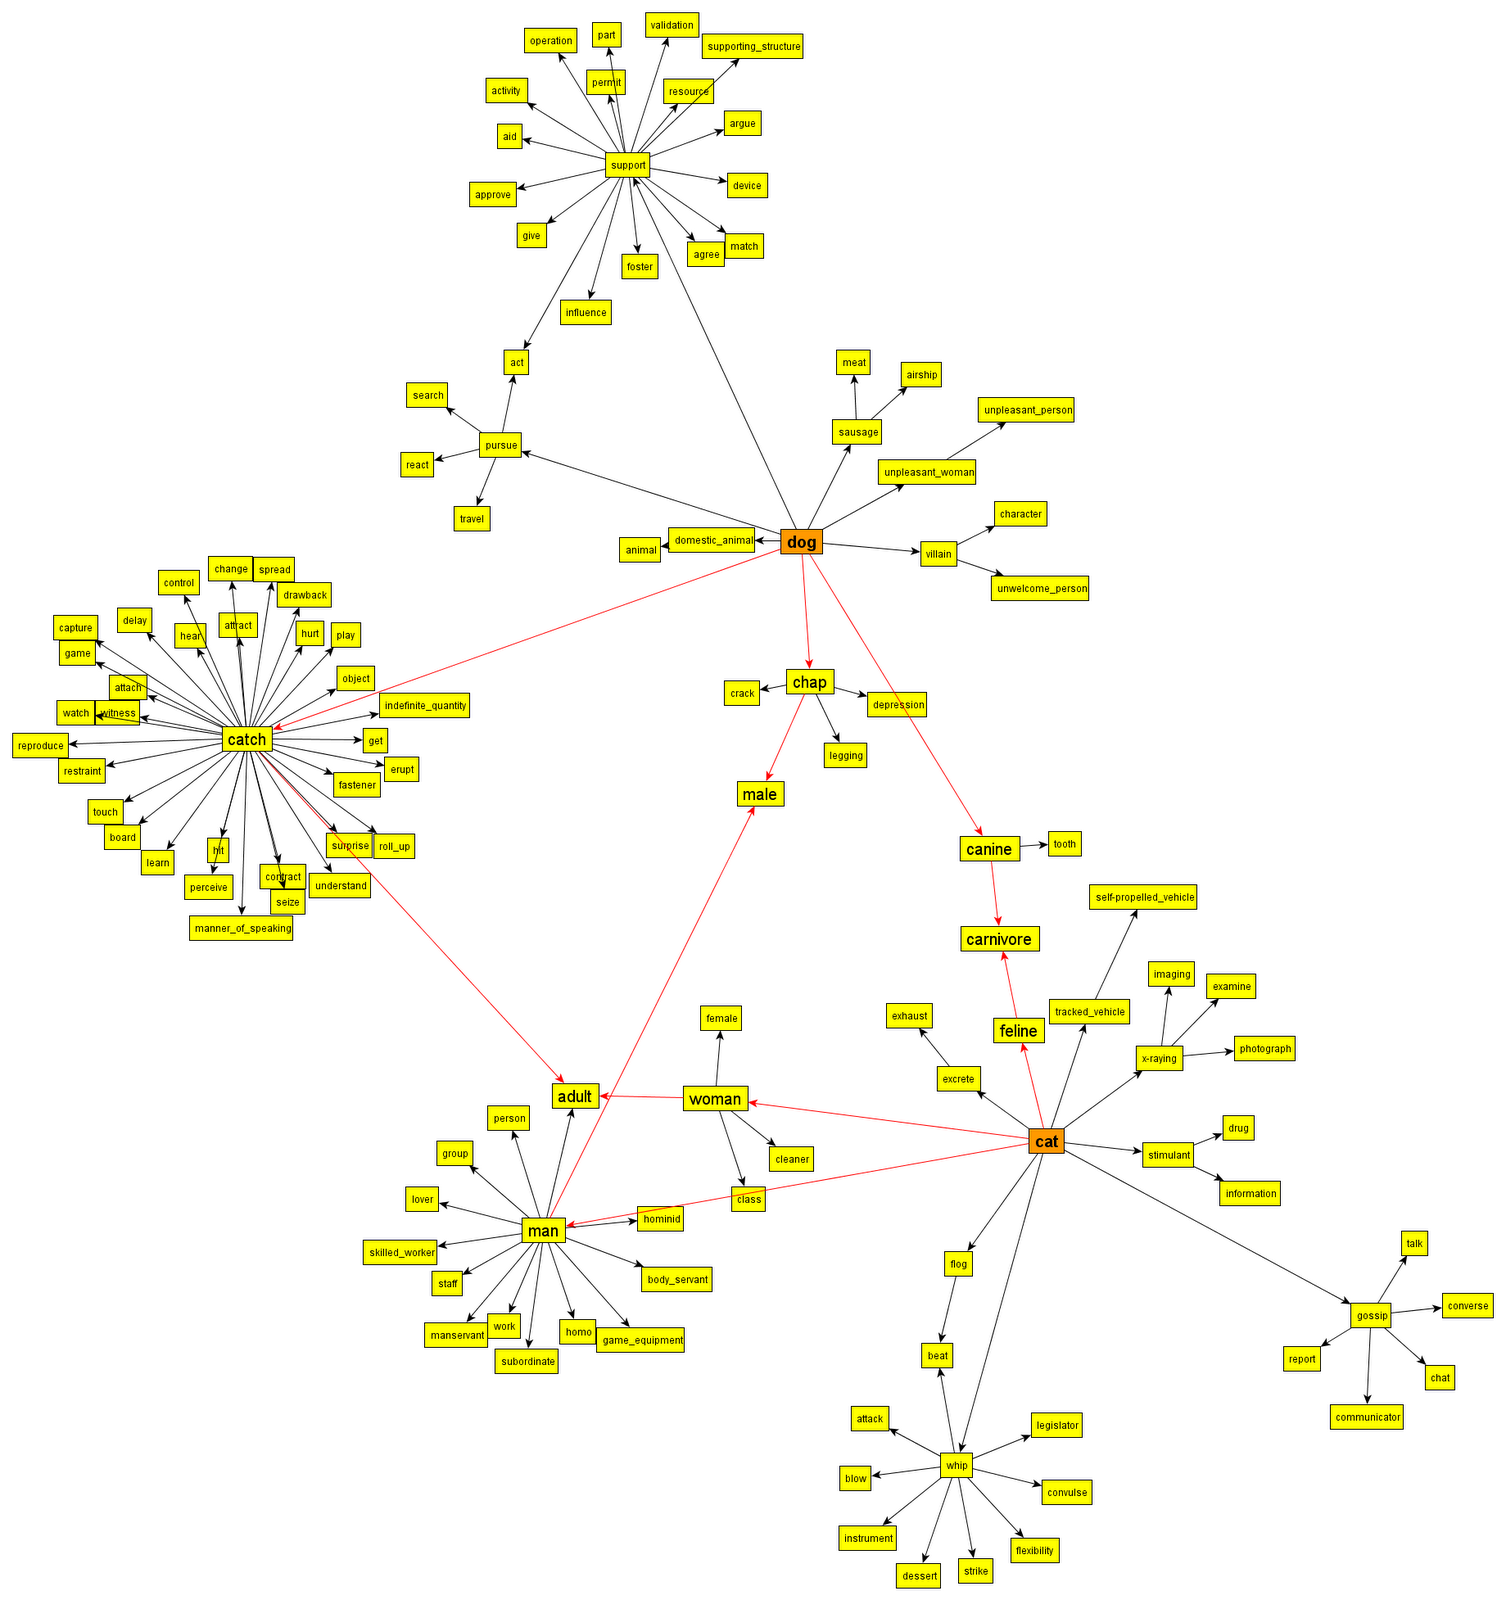
\includegraphics[width=0.65\textwidth]{figures/wordnet-big}
\label{fig:wordnet}
\end{figure}

{\footnotesize \url{http://geniferology.blogspot.com/2012/10/playing-with-wordnet.html}}
\end{frame}





\begin{frame}
\frametitle{A multilingual WordNet: BabelNet.org}

\begin{figure}
\centering
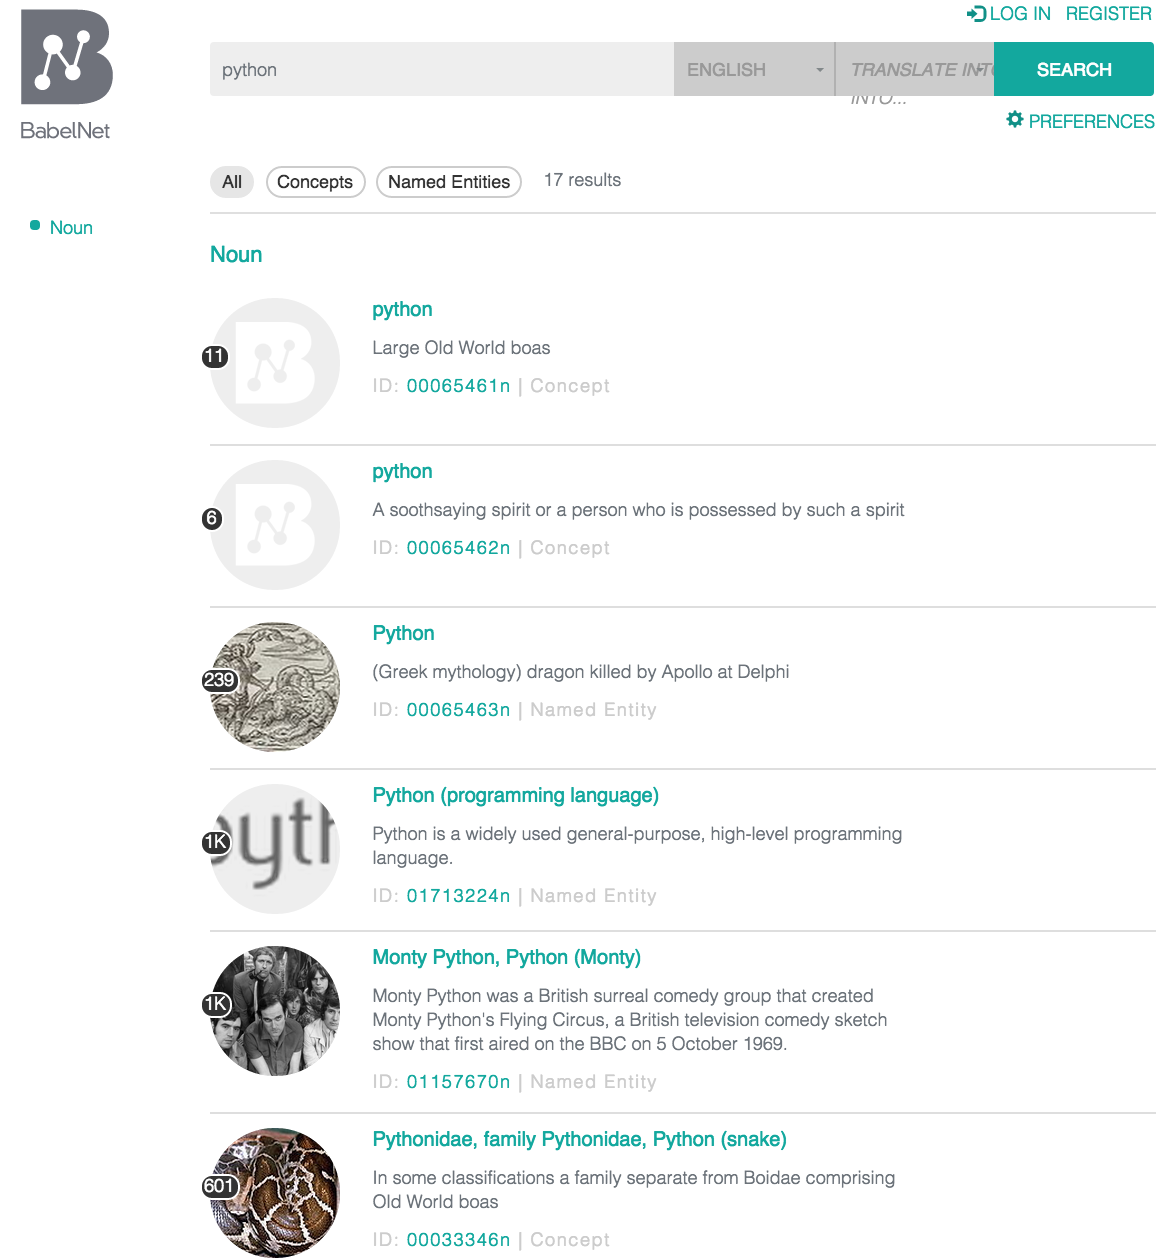
\includegraphics[height=0.7\textwidth]{./figures/babelnet1}
\end{figure}

\end{frame}




\begin{frame}
\frametitle{A multilingual WordNet: BabelNet.org}

\begin{figure}
\centering
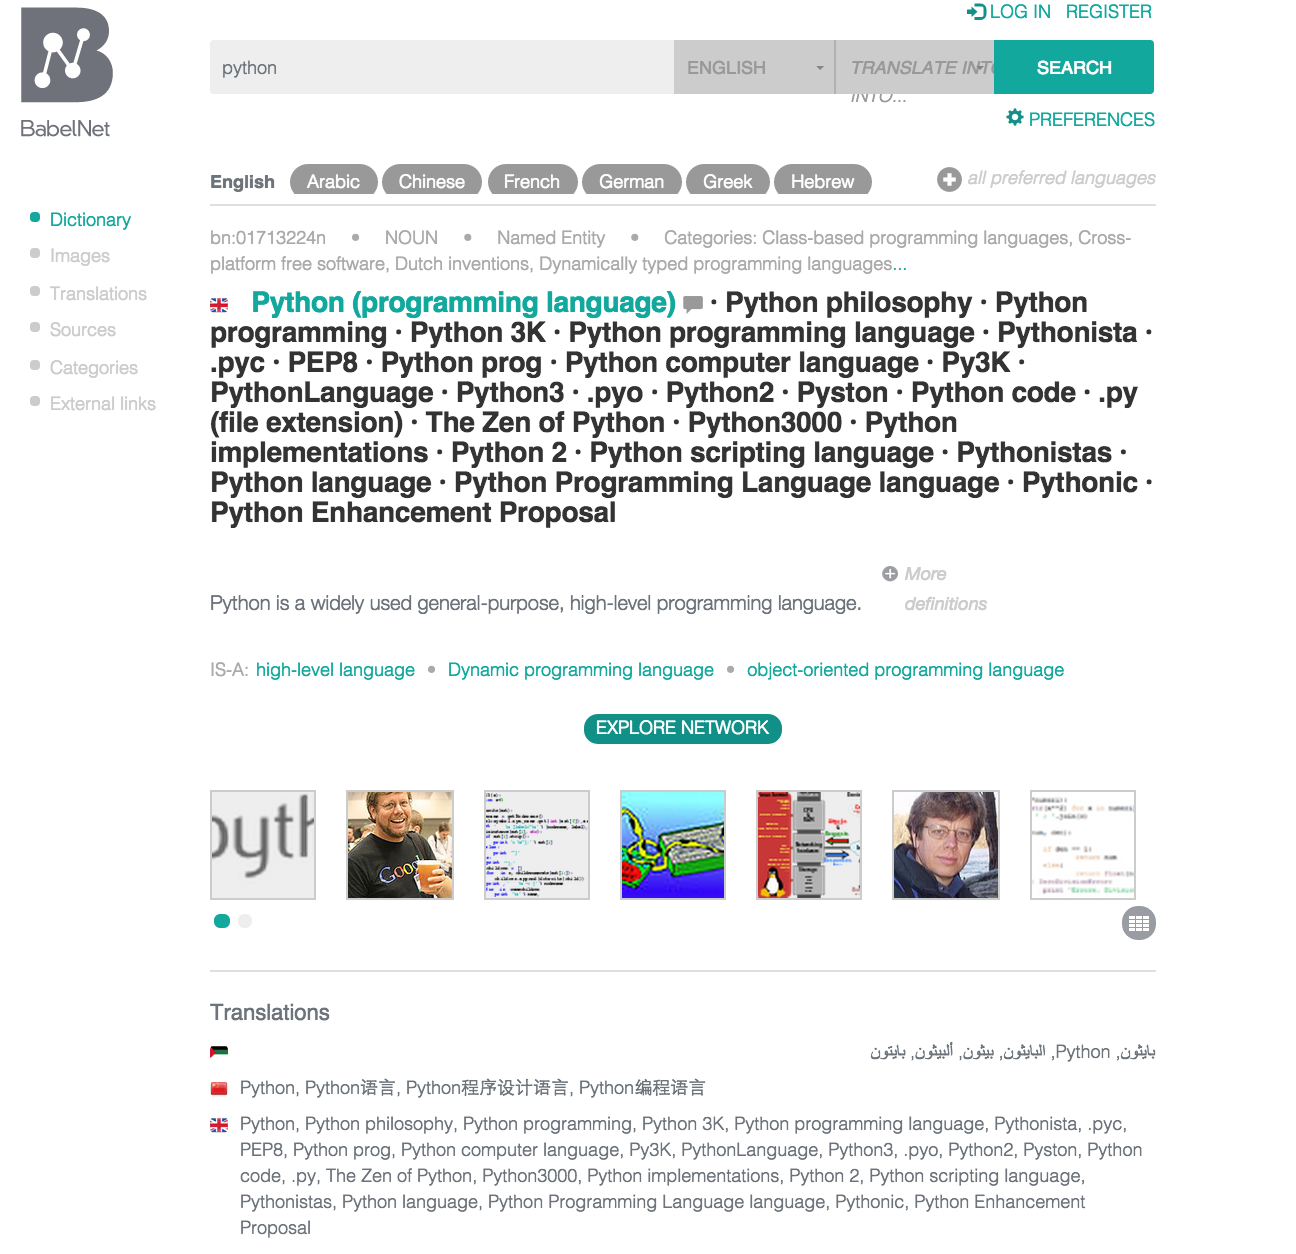
\includegraphics[height=0.7\textwidth]{./figures/babelnet2}
\end{figure}

\end{frame}





\begin{frame}
\frametitle{Semantic resources: ontology }

\begin{figure}
    \centering
        \includegraphics[width=1.0\textwidth]{../figures/ontology-new}
    \caption{ SUMO upper ontology: a part of the class hierarchy.}
    \label{fig:sumo}
\end{figure}
\end{frame}





\begin{frame}
\frametitle{Extraction of semantic resources from text }

\begin{figure}
\centering
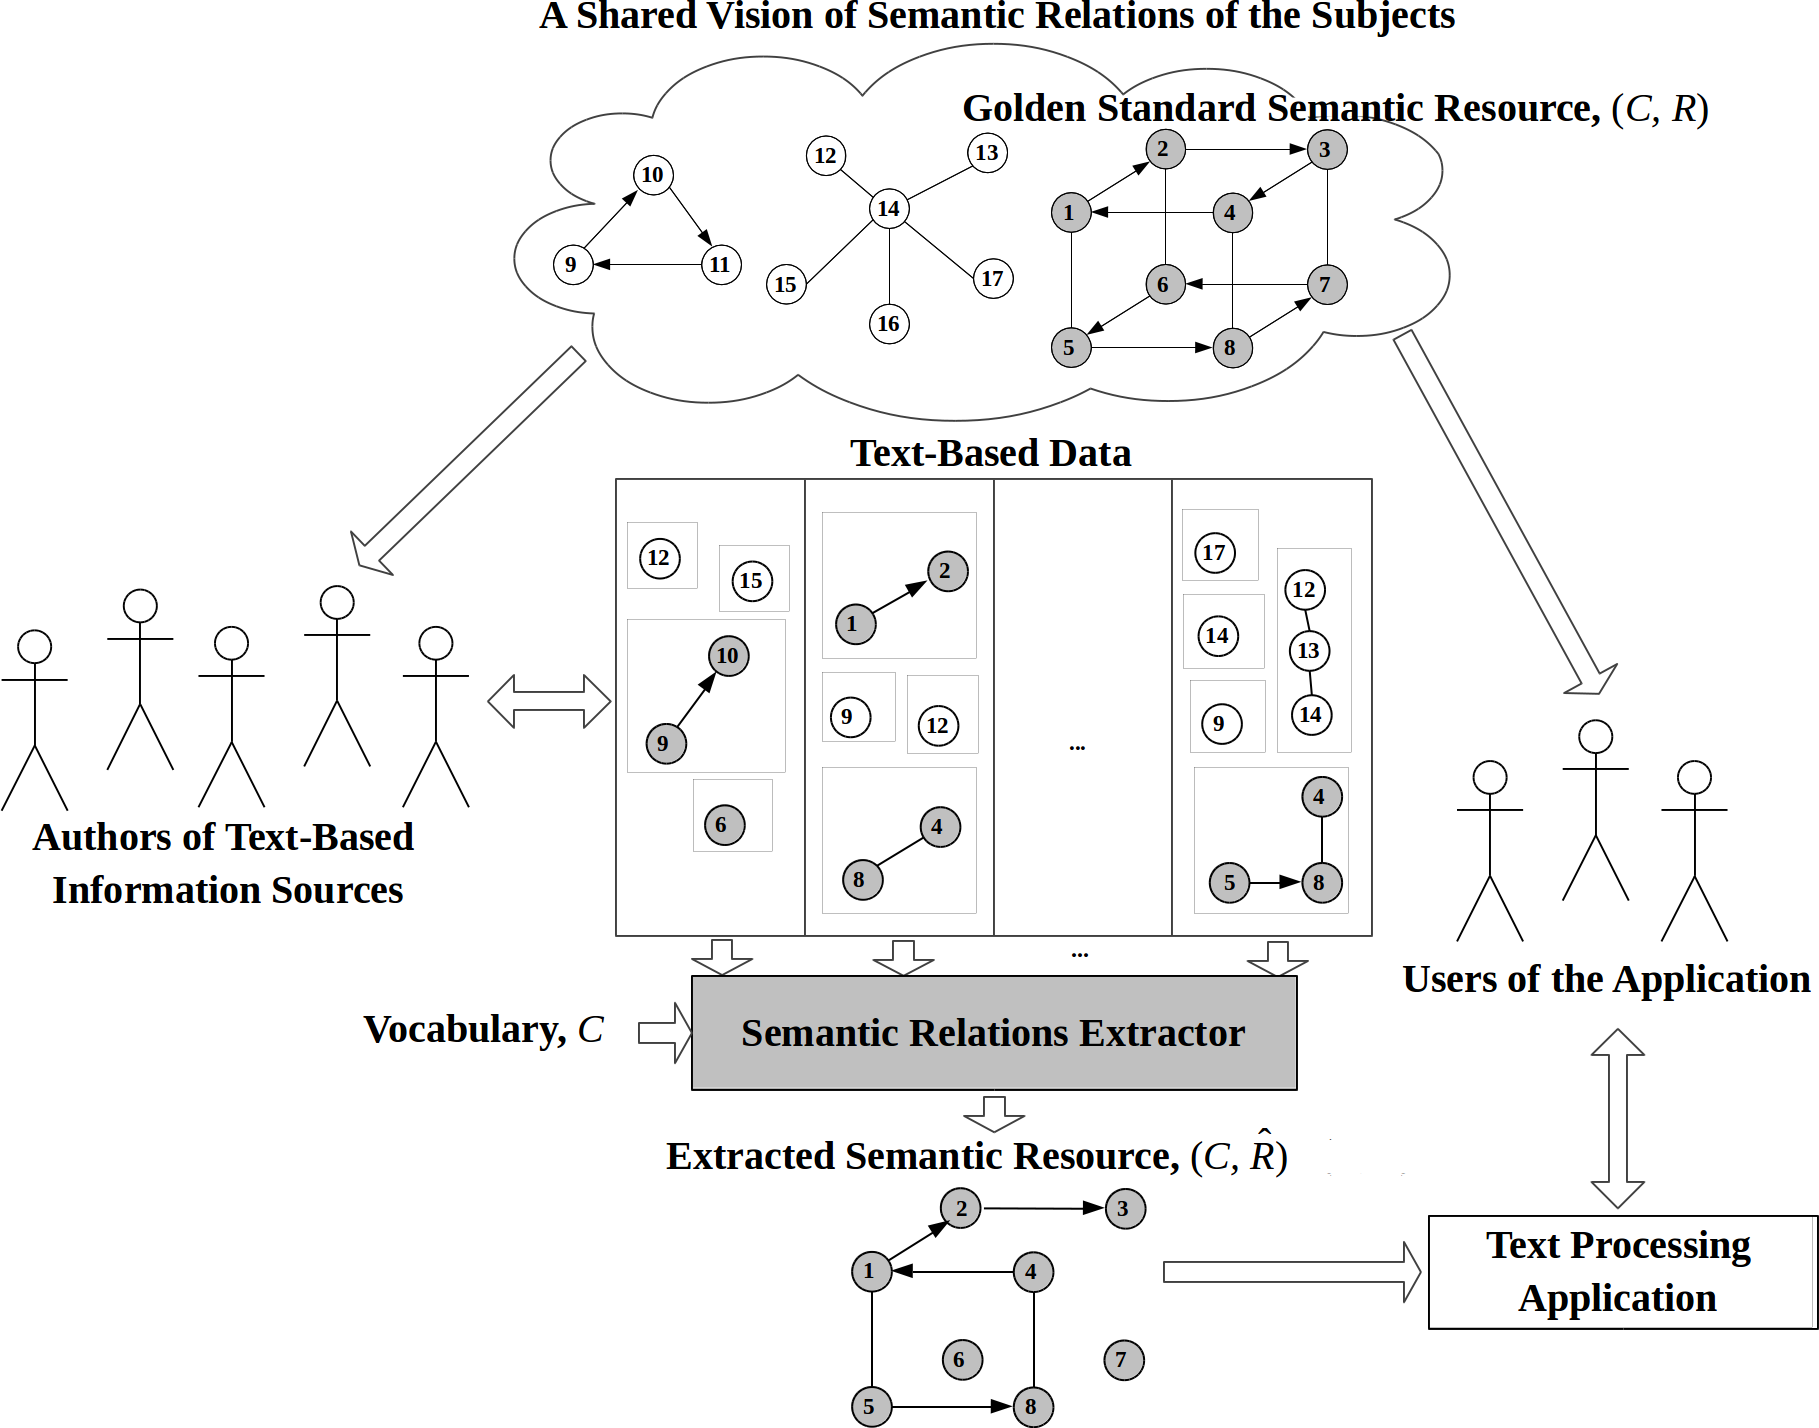
\includegraphics[width=0.8\textwidth]{../figures/extraction-3}

\label{fig:semantic-relations-extraction}
\end{figure}

\end{frame}






